\subsubsection{UC1-Registrazione account}
\begin{figure}[h] 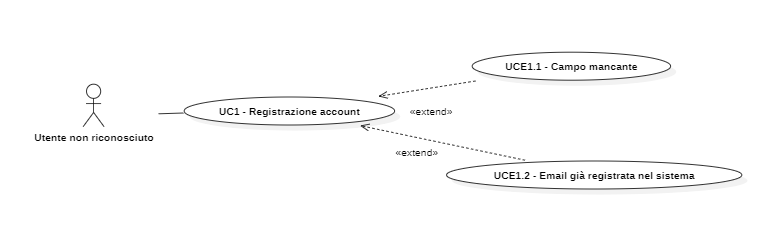
\includegraphics[scale=1]{uc01.png} \end{figure}
\begin{itemize}
    \item \textbf{Descrizione:} Il processo di registrazione creerà un \emph{account}$^{G}$ identificato da un ID univoco incrementale;
    \item \textbf{Attore principale:} Utente non riconosciuto;
    \item \textbf{Precondizioni:} L'utente è connesso al sistema;
    \item \textbf{Postcondizioni:} L'account dell'utente e le informazioni ad esso collegate, sono registrati nel sistema;
    \item \textbf{Scenario principale:}
        \begin{enumerate}
            \item L'utente sceglie l'opzione di registrazione di un account;
            \item Il sistema chiede all'utente di inserire una email ed una password;
            \item L'utente inserisce l'email e la password;
            \item L'utente conferma i valori inseriti;
            \item Il sistema comunica all'utente che la registrazione è andata a buon fine;
            \item L'utente visualizza un profilo di tipo cliente creato di default dal sistema.
        \end{enumerate}
    \item \textbf{Estensioni:}
        \begin{itemize}
                \item UCE1.1-Campo mancante;
                \item UCE1.2-Email già registrata nel sistema.
        \end{itemize}
\end{itemize}

\textbf{UCE1.1-Campo mancante}
\begin{itemize}
    \item \textbf{Descrizione:} Per effettuare la registrazione, deve essere inserito un valore sia per la password che per l'email;
    \item \textbf{Scenario alternativo:}
    \begin{enumerate}
        \item Al momento della conferma, il sistema rileva che uno dei campi (o entrambi) risulta non compilato;
        \item Il sistema comunica la natura dell'errore all'utente;
        \item L'utente visualizza i campi di mail e password con i valori inseriti precedentemente.
    \end{enumerate}
\end{itemize}

\pagebreak

\textbf{UCE1.2-Email già registrata nel sistema}
\begin{itemize}
    \item \textbf{Descrizione:} L'utente non può registrare con una email già presente nel sistema;
    \item \textbf{Scenario alternativo:}
    \begin{itemize}
        \item L'email inserita dall'utente al momento della registrazione risulta associata ad un account già registrato nel sistema;
        \item Il sistema comunica la natura dell'errore all'utente;
        \item L'utente è reindirizzato alla homepage di registrazione.
    \end{itemize}
\end{itemize}

\subsubsection{UC2-Login}
\begin{figure}[h] 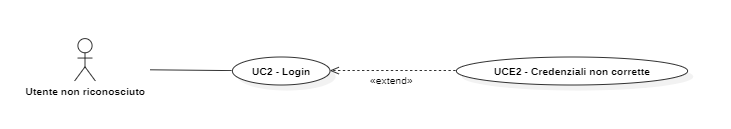
\includegraphics[scale=1]{uc02.png} \end{figure}
\begin{itemize}
\item \textbf{Attore principale:} Utente non riconosciuto;
\item \textbf{Precondizioni:} L'utente è connesso al sistema;
\item \textbf{Postcondizioni:} L'utente è autenticato presso il sistema;
\item \textbf{Scenario principale:}
\begin{enumerate}
    \item L'utente sceglie l'opzione di login;
    \item L'utente inserisce la sua password;
    \item L'utente inserisce la sua email;
    \item L'utente conferma i dati inseriti al sistema;
    \item Il sistema verifica l'esistenza di un account con i suddetti dati;
    \item L'utente visualizza la lista dei profili afferenti al suo account.
\end{enumerate}
    \item \textbf{Estensione:} UCE2-Credenziali non corrette.
\end{itemize}

\subsubsection{UCE2-Credenziali non corrette}
\textbf{Descrizione:} Il login può non andare a buon fine se l'email inserita dall'utente non è registrata
o la password non è corretta; per questioni di sicurezza, all'utente viene notificato un errore generico.
\textbf{Scenario secondario:}
\begin{enumerate}
    \item Dopo la conferma dei dati inseriti dall'utente, il sistema verifica che l'email non è presente nel sistema o che la password associata non è corretta;
    \item Il sistema comunica all'utente che le credenziali inserite non sono corrette;
    \item L'utente può riprovare ad effettuare il login, inserendo di nuovo l'email e la password.
\end{enumerate}
